%
% richtungsableitung.tex -- Richtungsableitung einer Funktion f(x,y)
%
% (c) 2024 Prof Dr Andreas Müller
%
\begin{figure}
\centering
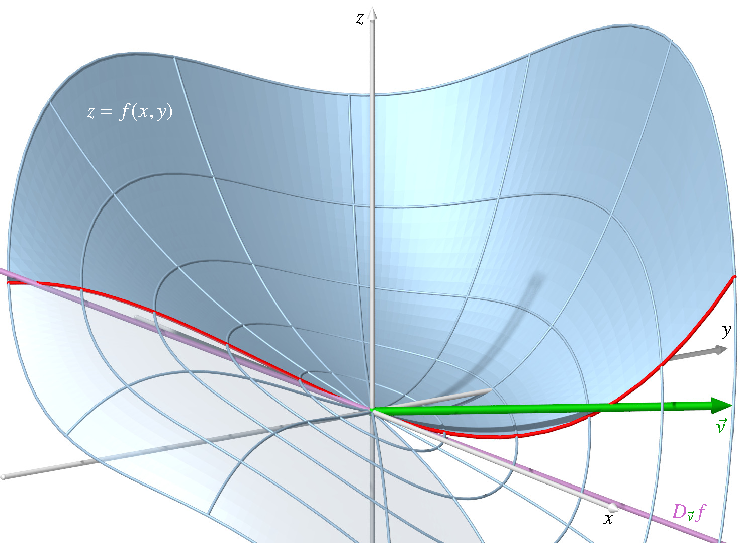
\includegraphics{chapters/010-fuvar/images/richtungsabl.pdf}
\caption{Definition der Richtungsableitung einer Funktion $f(x,y)$
zweier Variablen in Richtung des {\color{darkgreen}grünen}
Vektors ${\color{darkgreen}\vec{v}}$.
Die Richtungsableitung ist die Steigung der {\color{darkred}roten}
Schnittkurve der vertikalen Ebene mit Richtung ${\color{darkgreen}\vec{v}}$ 
und der Fläche des Graphen $z=f(x,y)$.
\label{buch:fuvar:richtungsableitung:fig:richtungsableitung}}
\end{figure}
